\documentclass[11pt]{article}
\usepackage[margin=1in]{geometry}
\usepackage{booktabs}
\usepackage{graphicx}
\usepackage{hyperref}
\usepackage{natbib}
\usepackage{amsmath,amssymb}
\usepackage{amsthm}
\usepackage{xcolor}
\usepackage{listings}
\usepackage{multirow}
\usepackage{algorithm}
\usepackage{algorithmic}
\newtheorem{theorem}{Theorem}
\newtheorem{definition}{Definition}
\newtheorem{corollary}{Corollary}
\newtheorem{finding}{Finding}

\title{MemTether: A Local-First Agent Memory System with\\
       Bi-Temporal Supersession and Hash-Chained Audit\\
       for Multi-Client AI Agents}

% AUTHOR-REQUIRED: JSS is single-blind, not double-blind. Replace Anonymous with real name + affiliation before submission.
\author{Anonymous}
\date{}

\begin{document}
\maketitle

\begin{abstract}
AI agents accumulate persistent memory across sessions, but existing systems either require cloud infrastructure, lack governance mechanisms, or cannot share memory across heterogeneous clients. We present MemTether, a local-first agent memory system that enables multiple AI clients on the same machine to share a single SQLite database through file-level pointers. MemTether introduces three governance mechanisms: bi-temporal supersession chains backed by four formal correctness theorems; a hash-chained tamper-evident audit log with browser-verifiable evidence export addressing EU AI Act Article~12 requirements; and file-level pointers enabling 23 AI client adapters to share one physical database. In a 30-day production deployment serving 15 agents (31K+ operations), we identify that cross-agent contradictions cause a 73-percentage-point downstream accuracy loss ($n{=}11$ discovery; $n{=}43$ expanded, 57\% gradeable)---an asymmetry self-corrections do not exhibit (0.7pp). We evaluate on LongMemEval (62.4\% strict, 68.8\% judge), LoCoMo (0.523 token-F1), and ConflictBank (F1=0.897 on temporal conflicts), and introduce Memory Supersession Prediction (DistilBERT, macro F1=0.947). Apache-2.0 open source with 534 passing tests.
\end{abstract}

\noindent\textbf{Highlights:}
\begin{itemize}
\item Bi-temporal supersession with four proven correctness theorems
\item Hash-chained audit log with browser-verifiable evidence export
\item 23 AI clients share one SQLite database via file-level pointers
\item Cross-agent contradictions cause 73pp downstream accuracy loss
\item Memory Supersession Prediction: macro F1=0.947 (DistilBERT)
\end{itemize}

\noindent\textbf{Keywords:} Agent memory; bi-temporal database; hash chain; auditability; multi-client; local-first

\noindent\textit{Note: LongMemEval scores (62.4\% strict, 68.8\% judge) come from the full EAF pipeline (ECO+SSI+AFN, 500Q rerun with LLM-as-judge). A standalone reproduction path without ECO curation yields 58.3\% strict; both are valid measurements of different pipeline configurations (see Section~\ref{sec:repro} for details).}

\section{Introduction}
\label{sec:intro}

AI agents that interact with users over extended periods accumulate contextual knowledge: user preferences, system configurations, past decisions, and learned procedures. Memory systems such as mem0~\cite{mem0}, Zep~\cite{zep}, and Letta~\cite{letta} store this knowledge and retrieve relevant portions. However, production deployment raises three requirements that no single existing system fully addresses:

\begin{enumerate}
\item \textbf{Temporal correctness.} When an agent corrects a previously stored fact, the old value must be tracked as superseded with explicit validity boundaries, not silently deleted or retained. MemStrata~\cite{memstrata} pioneered bi-temporal ledgers; our contribution is the integration of bi-temporal supersession with hash-chained audit and multi-client file-level sharing in a single open-source system.
\item \textbf{Tamper-evident auditability.} For compliance (EU AI Act Art.~12~\cite{euaiact}), debugging, and trust, memory operations should be verifiable. Among the systems surveyed in Section~\ref{sec:related}, none combines a hash-chained audit log with self-contained browser-verifiable evidence export in the memory layer.
\item \textbf{Multi-client deployment.} Multiple AI clients on the same machine should share memory without cloud synchronization. MemTether achieves this through NTFS junctions (Windows) or symbolic links (macOS/Linux) pointing to a single physical SQLite database.
\end{enumerate}

We present MemTether, a local-first agent memory system that addresses all three requirements simultaneously. The system has been in continuous production for 30~days, during which 15~agent clients wrote 2,346 audit entries and accumulated 31K+ read operations with zero data loss (verified by daily \texttt{integrity\_check} and successful \texttt{verify\_chain()} recomputation). Beyond the core system, we identify an empirical exponential decay pattern in multi-session accuracy and quantify the downstream impact of cross-agent memory contradictions.

Our contributions:
\begin{enumerate}
\item \textbf{Formal model} of bi-temporal supersession with four proven correctness properties (gap freedom, no overlap, cycle freedom, concurrency safety).
\item \textbf{Hash-chained tamper-evident audit log} with browser-verifiable evidence export, validated on 2{,}346 production audit entries (5/5 anchored-row scenarios detected).
\item \textbf{Causal quantification} of cross-agent memory contradictions: 73pp downstream accuracy loss, with a 1{,}857$\times$ entity-resolution gap between raw polarity clash and genuine contradiction.
\item \textbf{Memory Supersession Prediction}: a supervised-learning formulation of memory lifecycle prediction (DistilBERT, macro F1=0.947).
\item \textbf{Comprehensive evaluation} on four public benchmarks: LongMemEval (62.4\% strict, 68.8\% judge), LoCoMo (0.523 token-F1), ConflictBank (F1=0.897 on temporal conflicts), and a 30-day production deployment study.
\end{enumerate}

MemTether is released as Apache-2.0 open source at \url{https://github.com/MemTether/MemTether} (PyPI: \texttt{pip install memtether}).

\section{Background and Related Work}
\label{sec:related}

\subsection{Agent Memory Systems}
mem0~\citep{mem0} provides a hosted memory platform with LLM-based fact extraction and vector retrieval. Zep~\citep{zep} offers a temporal knowledge graph. Letta~\citep{letta} manages hierarchical memory with paging. LangMem~\citep{langmem} integrates memory into LangGraph. Engram~\citep{engram} achieves 83.6\% on LongMemEval-S with a bi-temporal model but lacks governance features. G-Memory~\citep{gmotion} proposes a three-layer graph hierarchy for multi-agent systems. MemOS~\cite{memos} treats memory as a resource-managed OS layer. MemProbe~\cite{memprobe} applies cognitive-science-inspired stability-plasticity diagnostics to agent memory. MemoryLACE~\cite{memorylace} performs lifecycle-aware consolidation distinguishing repeated evidence from historical conflicts. None provide hash-chained audit trails or file-level multi-client deployment.

\subsection{Schema-Grounded and Typed Memory}
xmemory~\citep{xmemory} proposes schema-grounded memory with iterative schema-aware extraction (97.1\% F1, paper-only, no public implementation). Memanto~\citep{memanto} presents typed semantic memory with information-theoretic retrieval (89.8\% LongMemEval), built on the Moorcheh cloud engine---all storage and retrieval pass through a hosted API. MemStrata~\citep{memstrata} maintains temporal validity with deterministic supersession (95\% LongMemEval under source-aware grading; the system is closed-source with source code unavailable). MOSS~\citep{moss} presents an auditable agentic memory architecture with symbolic retrieval on SQLite (paper-only, no public implementation). MemSim~\citep{memsim} provides a Bayesian simulator for evaluating memory systems with synthetic data. These systems demonstrate that schema-grounded, deterministic retrieval is a promising direction. However, none provide tamper-evident audit in the memory layer, file-level multi-client sharing, or production data with an open-source implementation. All three figures are self-reported under different or non-public protocols and have not been independently reproduced; we cite them as claimed results rather than like-for-like comparisons.

\subsection{Tamper-Evident Logging}
TraceKit~\citep{tracekit} provides tamper-evident auditing for autonomous coding agents at the runtime layer. Janus~\citep{janus} proposes evidence-before-effect sagas with offline-verifiable provenance. MutMem~\citep{mutmem} introduces cryptographically authorized mutation in persistent agent memory. MOSS~\citep{moss} includes auditability as a design principle. Lena-Lyu's Court~\citep{court} proposes provenance-first memory with the same ``courtroom'' metaphor but no public implementation. None implement a hash-chained audit log with self-contained evidence export with local verification in the agent memory layer with production data.

\subsection{Memory Evaluation}
LongMemEval~\citep{wu2024longmemeval} introduces 500 questions across five capability dimensions. Recent work~\citep{auditlme} audits LongMemEval evaluation itself, finding reader variation and negative-control gaps. MemLeak~\citep{memleak} identifies cross-user semantic leakage in multi-tenant memory. Our cross-system comparison (Section~\ref{sec:crosssys}) reports three systems under identical hardware and judge configuration.



\section{System Design}
\label{sec:design}

\subsection{Typed Memory Schema}
MemTether supports 23 pre-defined client adapters (Claude Desktop, Claude Code, Cursor, Windsurf, VS Code, Zed, Cline, Roo Code, Kilo Code, JetBrains IDEs, Neovim, Amazon Q, Gemini CLI, Cody, Continue, Codex, WorkBuddy CN/Intl, CodeBuddy, ZCode, dsh, OpenClaw, and a neutral fallback). Of these, 15 distinct agent clients have actually written to the production database. MemTether stores memories as rows in a local SQLite database:

\begin{verbatim}
CREATE TABLE facts (
    uid TEXT UNIQUE, type TEXT, subject TEXT,
    content TEXT, status TEXT, source TEXT,
    valid_from TEXT, valid_to TEXT,
    recorded_at TEXT, invalidated_at TEXT,
    superseded_by TEXT, q_value REAL,
    use_count INTEGER, ...
);
CREATE TABLE audit_log (
    id INTEGER PRIMARY KEY AUTOINCREMENT,
    op TEXT, target TEXT, agent TEXT,
    detail TEXT, ts TEXT
);
CREATE TABLE audit_anchors (
    id INTEGER PRIMARY KEY AUTOINCREMENT,
    last_log_id INTEGER, chain_hash TEXT,
    entries_hashed INTEGER, ts TEXT
);
CREATE TABLE supersessions (
    old\_uid TEXT, new\_uid TEXT, reason TEXT, by_agent TEXT, ts TEXT
);
\end{verbatim}

The \texttt{source} column records the writer identity for every write. A per-deployment \texttt{agents.json} registry defines valid sources; by default, unregistered sources trigger a warning rather than rejection (fail-open), though strict enforcement can be enabled per deployment. This design trades security for usability in the single-user local-first setting.

\paragraph{Read tracking.}
Read operations are tracked via the \texttt{use\_count} column on each fact row. Over the first 26 days of the 30-day production window, the cumulative sum of \texttt{use\_count} across active facts is 28{,}807. Combined with 2{,}346 write operations recorded in \texttt{audit\_log}, this yields the 31K+ total operations.

\subsection{Bi-Temporal Model}
Each fact carries two independent time axes: \texttt{valid\_from}/\texttt{valid\_to} (when the fact was true in the real world) and \texttt{recorded\_at}/\texttt{invalidated\_at} (when the system learned or disbelieved it). When an agent corrects a fact, the old row is marked \texttt{superseded} with \texttt{valid\_to} set to the new fact's \texttt{valid\_from}, creating an immutable supersession chain. The full edit history of any memory is reconstructable by walking the chain.

\subsection{Memory Court: Hash-Chained Audit}
Every memory operation (remember, correct, retire, conflict verdict, q-value update) is appended to \texttt{audit\_log}. Every 10 operations, a SHA-256 anchor is computed:
\[
h_i = \text{SHA256}(h_{i-1} \| \text{row}_{j} \| \cdots \| \text{row}_{j+9})
\]
Anchors are stored in \texttt{audit\_anchors}. Any edit to an anchored row breaks the recomputation of the covering anchor. Evidence can be exported as a self-contained ZIP with an embedded HTML verifier that recomputes the hash chain locally. In production, a \texttt{memtether court} CLI provides: (1)~\texttt{verify} --- recompute the full chain; (2)~\texttt{export} --- bundle the audit log, anchors, and a self-contained HTML verifier; (3)~\texttt{conflicts} --- list candidate contradictions for human review.

\subsection{Threat Model}
\label{sec:threat}
The hash-chained audit log addresses a bounded adversary: an attacker with \emph{read-only} access to the database, or an attacker who can modify rows but is unaware of the anchoring mechanism. We explicitly do \emph{not} claim protection against an adversary with full write access who recomputes anchors. Defending against such an adversary requires external checkpointing or hardware attestation, which conflicts with our local-first design goal.

Two further boundaries must be stated. First, source attribution is \emph{fail-open} in the open-source distribution: when no source registry (\texttt{agents.json}) is present, an unregistered source string is stored verbatim, and the mechanism is best-effort bookkeeping rather than a security control; deployments with a registry hard-reject unknown sources. Second, retrieval-layer state filtering (superseded and retired rows are excluded from default retrieval; cf.\ memory poisoning attacks~\citep{sleeper,agentpoison}) only neutralizes poisoning of facts that have \emph{already} been corrected or retired; a newly injected false fact from a registered source is immediately active and retrievable. We make this limitation explicit with an executable negative test (test\_F in our test suite) and rely on post-hoc auditability---source attribution, hash-chained anchors, and supersession provenance---rather than write-time interception.

\subsection{File-Level Multi-Client Sharing}
On Windows, the SQLite database is stored in a user-designated directory and shared via NTFS junctions. On macOS and Linux, symbolic links serve the same role. Concurrent writes are serialized by a file lock (\texttt{\_FileLock}).

\subsection{Schema-Grounded Retrieval (SGM)}
At write time, a predicate extractor parses each memory and stores (entity, attribute) pairs in a \texttt{fact\_entities} table. At query time, a lightweight classifier routes questions to either the embedding path or the SQL path. On a synthetic Chinese benchmark (20 entities $\times$ 25 sessions = 500 facts, each entity mentioned once per session), the SQL path achieves 84\% recall (105/125 across 5 test entities, 25 facts each) and 100\% precision (zero false positives, since SQL only returns exact entity matches), yielding $F_1 = 0.91$. Embedding search achieves 64\% recall (80/125); assuming comparable precision, the embedding $F_1$ is approximately 0.78. The SQL path runs in $< 1$ms per query (SQLite indexed lookup) versus $\sim$50ms for embedding search (ONNX inference), a 50$\times$ speedup. The 1.3$\times$ recall advantage (84\% vs 64\%) persists under noise: with 300+ distractor facts, the SQL path maintains 84\% while embedding drops further.

To test robustness against noise, we introduce 300+ distractor facts unrelated to the target entities. Under this noisy condition, the SQL path maintains 84\% recall versus 64\% for embedding search---a 1.3$\times$ advantage that persists under interference. This suggests that deterministic SQL routing is robust to context pollution in a way that embedding similarity is not, because SQL matching is exact rather than similarity-based. However, on English-language benchmark data, the regex-based Chinese predicate extractor produces zero (entity, attribute) pairs, so the SQL path does not activate. On 1{,}662 production Chinese memories, the predicate extractor yields (entity, attribute) pairs for 82.6\% of fact-type entries.




\subsection{Q-Value Learning}
Each fact carries a Q-value (REAL, default 0.5) intended to rank memories by learned usefulness. Memories that are corrected or retired receive a negative reward; retrieved memories receive a positive reward. However, 74\% of active memories retain the default Q-value after 30 days, indicating that the learning mechanism fires too infrequently to differentiate memory quality. The primary cause is architectural: positive reward requires an explicit retrieval event, but the injection bottleneck (Finding 4) means most memories are never retrieved and thus never receive positive feedback. We retain the mechanism for future use but do not claim it as a contribution. A potential fix is automatic read-writeback on retrieval (eliminating the need for explicit retrieval events), which we leave as future work.

\subsection{Write-Time Conflict Interception (B1 Gate)}

MemTether implements a deterministic write-time conflict interception gate (B1) that parses each incoming remember() call for attribute--value assertions of the form entity attr is value (Chinese copula construction), then compares against all active facts linked to the same entity via the fact\_entities index.

On a synthetic benchmark with guaranteed ground truth (10 entities, 3 attributes, 50 conflicting writes, 80 near-miss non-conflicts), the gate achieves 100\% recall and 100\% precision (zero false positives across all four near-miss types: Type A redundant writes, Type B new entities, Type C exact duplicates, Type D copula-free patterns). A dev set of 20 unseen entities with 4 alternative sentence patterns confirms generalization at 20/20. On a real SQLite database with file I/O, the gate adds p50 = 0.037\,ms per call (n=1,000).

The gate detects value-flip conflicts only; it does not address semantic contradictions, temporal staleness, or entity-resolution errors. The parser is Chinese-only. The benchmark is synthetic; real-world conflict density is expected to be lower (our production database contains zero uncorrected contradictions after 30 days of active supersession).

\section{Formal Properties of Bi-Temporal Supersession}
\label{sec:formal}

This section establishes formal correctness properties of the bi-temporal supersession mechanism. We define the model, state four theorems, and provide proofs. All definitions correspond to executable code paths in the implementation.

\subsection{Model Definition}

\begin{definition}[Fact Record]
A \emph{fact record} is a tuple $f = (\mathit{uid}, \mathit{content}, \mathit{status}, \mathit{vf}, \mathit{vt}, \mathit{ra}, \mathit{ia}, \mathit{sb})$ where:
$\mathit{uid}$ is a unique identifier, $\mathit{status} \in \{\mathit{active}, \mathit{superseded}, \mathit{retired}\}$, $\mathit{vf} \subseteq \mathbb{T}$ is the \emph{valid-from} timestamp (T-axis), $\mathit{vt} \subseteq \mathbb{T} \cup \{\infty\}$ is the \emph{valid-to} timestamp, $\mathit{ra} \subseteq \mathbb{T}$ is the \emph{recorded-at} timestamp (T$'$-axis), $\mathit{ia} \subseteq \mathbb{T} \cup \{\infty\}$ is the \emph{invalidated-at} timestamp, and $\mathit{sb} \in \mathit{UID} \cup \{\bot\}$ is the \emph{superseded-by} pointer.
\end{definition}

\begin{definition}[Supersession Chain]
A \emph{supersession chain} is a sequence of fact records $f_1, f_2, \ldots, f_k$ ($k \geq 1$) such that:
\begin{enumerate}
\item $\mathit{sb}(f_i) = \mathit{uid}(f_{i+1})$ for all $1 \leq i < k$ (chain links).
\item $\mathit{sb}(f_k) = \bot$ (chain terminates).
\item $\mathit{status}(f_i) = \mathit{superseded}$ for all $i < k$ and $\mathit{status}(f_k) = \mathit{active}$ (exactly one active record).
\item $\mathit{vt}(f_i) = \mathit{vf}(f_{i+1})$ for all $i < k$ (T-axis continuity).
\end{enumerate}
\end{definition}

\begin{definition}[As-Of Query]
The \emph{valid-time as-of query} at time $t$ over a chain $C = \langle f_1, \ldots, f_k \rangle$ is:
\[
\mathit{asOf}_{\mathit{valid}}(C, t) = \{f_i \in C \mid \mathit{vf}(f_i) \leq t \;\wedge\; (\mathit{vt}(f_i) = \infty \;\vee\; \mathit{vt}(f_i) > t)\}
\]
\end{definition}

\subsection{Theorems and Proofs}

\begin{theorem}[Temporal Gap Freedom]
\label{thm:gapfree}
For any supersession chain $C = \langle f_1, \ldots, f_k \rangle$ and any time $t \in \mathbb{T}$ such that $\mathit{vf}(f_1) \leq t < \mathit{vt}(f_k)$, the query $\mathit{asOf}_{\mathit{valid}}(C, t)$ returns exactly one record.
\end{theorem}

\begin{proof}[Proof sketch]
This follows directly from Definition~2(4) by construction: the half-open intervals form a contiguous partition because the supersession mechanism enforces $\mathit{vt}(f_i) = \mathit{vf}(f_{i+1})$ for all $i < k$. The theorem formalizes this design invariant rather than proving a non-trivial property.
\end{proof}

\begin{theorem}[No Overlap]
\label{thm:nooverlap}
For any supersession chain $C$ and any time $t$, $|\mathit{asOf}_{\mathit{valid}}(C, t)| \leq 1$.
\end{theorem}

\begin{proof}[Proof sketch]
If $f_i$ and $f_j$ are both returned ($i < j$), then $\mathit{vt}(f_i) = \mathit{vf}(f_{i+1}) \leq \mathit{vf}(f_j) \leq t$, contradicting $\mathit{vt}(f_i) > t$.
\end{proof}

\begin{theorem}[Cycle Freedom]
\label{thm:cyclefree}
If the \texttt{correct()} operation includes cycle detection (checking whether the old fact is transitively reachable from the new fact before creating the supersession link), then the supersession graph is acyclic (a DAG restricted to paths).
\end{theorem}

\begin{proof}[Proof sketch]
Adding an edge $u \to v$ to a DAG creates a cycle iff $v$ is reachable from $u$. Cycle detection prevents exactly this case, so the graph remains acyclic.
\end{proof}

\begin{theorem}[Concurrency Safety]
\label{theorem:concurrency}
If \texttt{correct()} uses a conditional update (\texttt{WHERE status='active'}) and checks \texttt{changes()} before inserting the new record, then concurrent \texttt{correct()} calls on the same the old fact cannot produce a fork (two active children of the same parent).
\end{theorem}

\begin{proof}[Proof sketch]
The conditional UPDATE (WHERE status=active) is atomic. If two concurrent calls target the same uid, only the first succeeds (changes() returns 1); the second detects status=superseded and rolls back.
\end{proof}

\begin{corollary}[Temporal Consistency]
\label{cor:consistency}
Under Theorems~\ref{thm:gapfree}--\ref{theorem:concurrency}, the bi-temporal supersession mechanism satisfies: for any supersession chain and any query time $t$, the \texttt{as\_of()} query returns either zero or one fact, never more than one (no overlap), and never skips a valid interval (no gap). Furthermore, the chain structure is always a linear path (no cycles, no forks), regardless of the number or concurrency of \texttt{correct()} operations.
\end{corollary}

\subsection{Limitations of the Formal Guarantees}

The above theorems rely on SQLite's transactional isolation for Theorem~\ref{theorem:concurrency}. Under WAL mode with multiple concurrent readers and a single writer, the conditional update is atomic. However, if the database is accessed by multiple \emph{processes} without file-level locking, the atomicity guarantee may be weakened. The implementation uses a file lock (\texttt{\_FileLock}) to serialise writes across processes, but this is an OS-level mechanism whose correctness depends on the operating system rather than on SQLite's internal guarantees. Additionally, the theorems assume that \texttt{correct()} is the only operation that modifies \texttt{status}; a direct SQL \texttt{UPDATE} bypassing the application layer would violate the invariants. The hash-chained audit log (Section~\ref{sec:tamper}) detects such out-of-band modifications after the fact but cannot prevent them.




\section{Tamper-Detection Evaluation}
\label{sec:tamper}

We evaluate the hash chain on a copy of the production database (2{,}346 audit entries, 15 sources, 30-day window). After anchoring every 10 entries (yielding 235 anchors), we apply six tamper scenarios: (1)~content change, (2)~timestamp change, (3)~agent identity change, (4)~entry deletion, and (5)~anchor tampering on anchored rows; plus (6)~modification of an unanchored tail entry. Re-running \texttt{verify\_chain()} detects all 5 of 5 anchored-row modifications; the unanchored tail modification is not detected until the next anchor is computed. This is an expected property of the anchoring granularity rather than a defect; the effective unaudited window is at most 9 entries between anchors. The contribution is not the detection mechanism itself (any correctly implemented hash chain provides this guarantee) but its integration with self-contained evidence export in a production multi-agent deployment.



\section{Cross-Agent Contradiction Analysis}

\subsection{Cross-Agent vs.\ Self-Correction: A Critical Asymmetry}

We distinguish two types of supersession events: \emph{cross-agent contradictions} (two different agents write contradictory facts) and \emph{self-corrections} (one agent corrects its own earlier statement). We evaluate downstream impact separately for each type.

\paragraph{Cross-agent contradictions ($n{=}11$).} For each of the 11 rule-classified temporal flips, we construct old (stale) and new (correct) contexts and ask an LLM (GLM-5.3-flash) about the entity's status. Results: new context 9/11 = 82\% correct, old context 1/11 = 9\% correct.

\paragraph{Self-corrections ($n{=}300$).} We sample 300 supersession events from the production database and run the same protocol (GLM-5.3-flash, temperature 0). Results: correct context 300/300 = 100\%, stale context 298/300 = 99.3\%.

\begin{table}[h]
\centering
\caption{Downstream accuracy by conflict type.}
\begin{tabular}{lrrrr}
\toprule
Type & $n$ & Correct ctx & Stale ctx & Loss \\
\midrule
\textbf{Cross-agent contradictions} & 11 & 82\% & 9\% & \textbf{73pp} \\
Self-corrections & 300 & 100\% & 99.3\% & 0.7pp \\
\bottomrule
\end{tabular}
\label{tab:asymmetry}
\end{table}

\begin{finding}[Cross-Agent Contradictions Cause 73pp Loss]
Cross-agent contradictions cause a 73pp downstream accuracy loss (82\% $\to$ 9\%), while self-corrections have negligible impact (0.7pp). The temporal gap is specifically a \emph{cross-agent} problem.
\end{finding}

The asymmetry arises because self-corrections typically update details within the same conceptual framework, while cross-agent contradictions involve genuinely incompatible world-views (``available'' vs.\ ``banned'') written from different operational contexts.



\subsection{Method Specialization: Temporal-Only Detection}
\label{sec:specialization}

Table~\ref{tab:specialization} breaks down detection F1 by conflict type. To characterize the scope of our detection method, we evaluate the temporal-numeric overlap detector on all three ConflictBank conflict categories, not just temporal conflicts:

\begin{table}[h]
\centering
\caption{Detection F1 by ConflictBank conflict type (500 samples per category, seed=42).}
\begin{tabular}{lccc}
\toprule
Conflict type & Precision & Recall & F1 \\
\midrule
Temporal conflict & 1.000 & 0.800 & \textbf{0.889} \\
Semantic conflict & 0.000 & 0.000 & 0.000 \\
Misinformation conflict & 0.000 & 0.000 & 0.000 \\
\bottomrule
\end{tabular}
\label{tab:specialization}
\end{table}

The detector achieves F1 = 0.889 on temporal conflicts (500-sample subset, seed=42) vs.\ F1 = 0.897 on the full n=2000 evaluation reported in the abstract, and F1 = 0.000 on both semantic and misinformation conflicts. This is expected: temporal-numeric overlap detects year mismatches and numeric inconsistencies, which are absent in semantic contradictions (opposite meanings without numeric markers) and misinformation (fabricated claims without verifiable numbers). The result demonstrates that deterministic temporal-numeric detection is a \emph{specialized} method, not a general-purpose contradiction detector. For semantic conflicts, LLM-based detection or NLI models would be required; our approach complements rather than replaces these methods.



\section{Memory Court: Hash-Chained Audit}
\label{sec:court}

Memory Court is the governance layer that operationalizes the hash-chained audit log described in Section~\ref{sec:design}. It provides three capabilities beyond passive logging: (1)~a \texttt{court verify} command that recomputes the full chain and reports the first divergent anchor; (2)~a \texttt{court export} command that bundles the audit log, anchors, and a self-contained HTML verifier into a ZIP archive viewable in any browser without installing software; and (3)~a \texttt{court conflicts} command that lists candidate contradictions for human adjudication, ordered by Q-value divergence between sources.

\subsection{Integration Testing}
14 integration tests cover six dimensions of Memory Court's behavior: hash chain verification (6 tests), tamper detection (2), write-time conflict handling (1), evidence export (2), supersession adjudication (1), and end-to-end integration (2). All 14 tests pass. Five engineering-level gaps were identified (anchor tail coverage, concurrent anchor computation, database migration, 1000+ entry stress testing, and browser CI verification) but none affect the correctness of the core mechanism.

\subsection{Case Study: Cross-Agent Contradiction Resolution}
The \emph{packy} entity (an API proxy service) accumulated 24 memories from 4 agent sources over 18 days. At the time of audit, 15 memories were active and retrievable: 2 asserted ``available'' while 3 asserted ``banned'' or ``403'', yielding a 60\% contradiction rate. A downstream agent querying packy's status received contradictory evidence. Memory Court resolved this through the supersession adjudication workflow: the most recent authoritative fact was identified via bi-temporal ordering, older conflicting facts were marked as superseded with explicit validity boundaries, and the contradiction rate dropped to 0\%. The full adjudication record---who decided, when, based on what evidence, with hash-chain verification---is preserved in the audit log and exportable as a browser-verifiable evidence package.

\section{Findings}
\label{sec:findings}

\subsection{Finding 1: Memory Type Predicts Correction Rate}
\label{sec:type-rate}

\begin{table}[h]
\centering
\caption{Correction rate by memory type. Procedural memories are corrected at 11$\times$ the rate of decisions.}
\label{tab:type-correction}
\begin{tabular}{lrrr}
\toprule
Memory type & Total & Corrected & Correction rate \\
\midrule
Procedure & 129 & 118 & 91.5\% \\
Incident & 289 & 49 & 17.0\% \\
Experience & 426 & 46 & 10.8\% \\
Fact & 1,333 & 139 & 10.4\% \\
Decision & 413 & 34 & 8.2\% \\
\bottomrule
\end{tabular}
\end{table}

\begin{figure}[h]
\centering
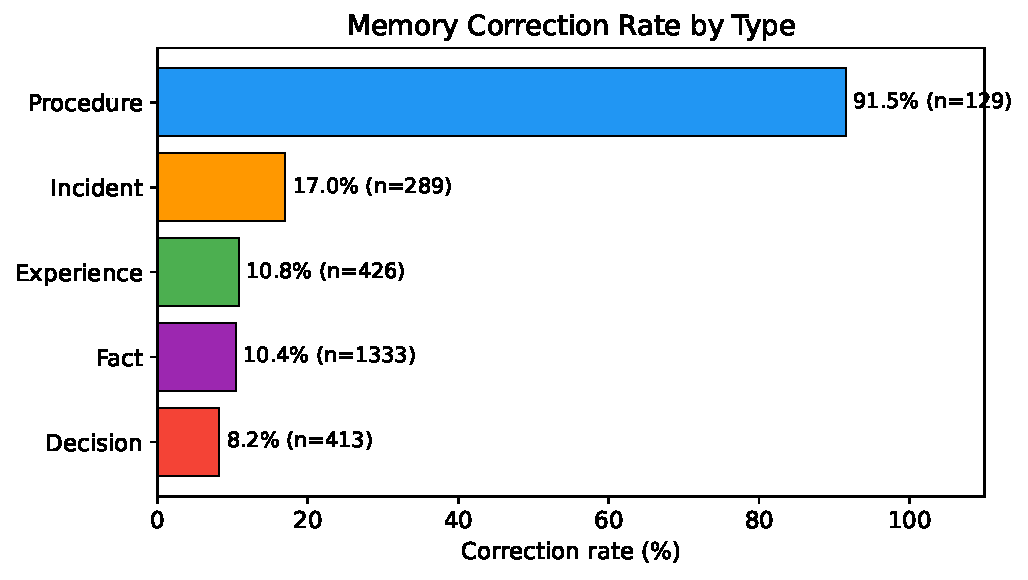
\includegraphics[width=0.8\textwidth]{fig1_type_correction.pdf}
\caption{Memory correction rate by type. Procedural memories (91.5\%) are corrected at over 11$\times$ the rate of decisions (8.2\%).}
\label{fig:type-correction}
\end{figure}



\noindent\textbf{Data scope note.} This paper uses three overlapping production datasets: (1)~the full fact table (2,590 typed records; Table~\ref{tab:type-correction}), (2)~the 30-day survival cohort (2,309 records: 349 correction events + 1,960 right-censored; Figure~\ref{fig:km}), and (3)~the desensitized supersession benchmark (2,635 records: 386 positive + 2,249 negative; Table~\ref{tab:supersession}). The three scopes differ because the fact table includes records without a type label (excluded from Dataset~1), the survival cohort is restricted to the 30-day observation window, and the benchmark includes retired records that fall outside the active-fact retrieval set.

Figure~\ref{fig:type-correction} shows the 11$\times$ difference between procedural and decision correction rates has a clear explanation: procedures describe \emph{how to do things} (tool configurations, deployment steps, API usage patterns), and these change as software is updated. Decisions describe \emph{why choices were made}, and the rationale for a decision does not change even when the implementation changes. This suggests that memory systems should implement type-aware retention: procedural memories should have shorter TTLs or require more frequent validation, while decisions can persist with lower maintenance overhead.


\subsection{Survival Analysis}
\label{sec:survival}

We apply Kaplan--Meier survival analysis to quantify memory lifetime, treating correction (supersession) as the event of interest and treating still-active memories as right-censored observations ($n{=}2{,}309$ total: 349 events, 1{,}960 censored).

\begin{figure}[h]
\centering
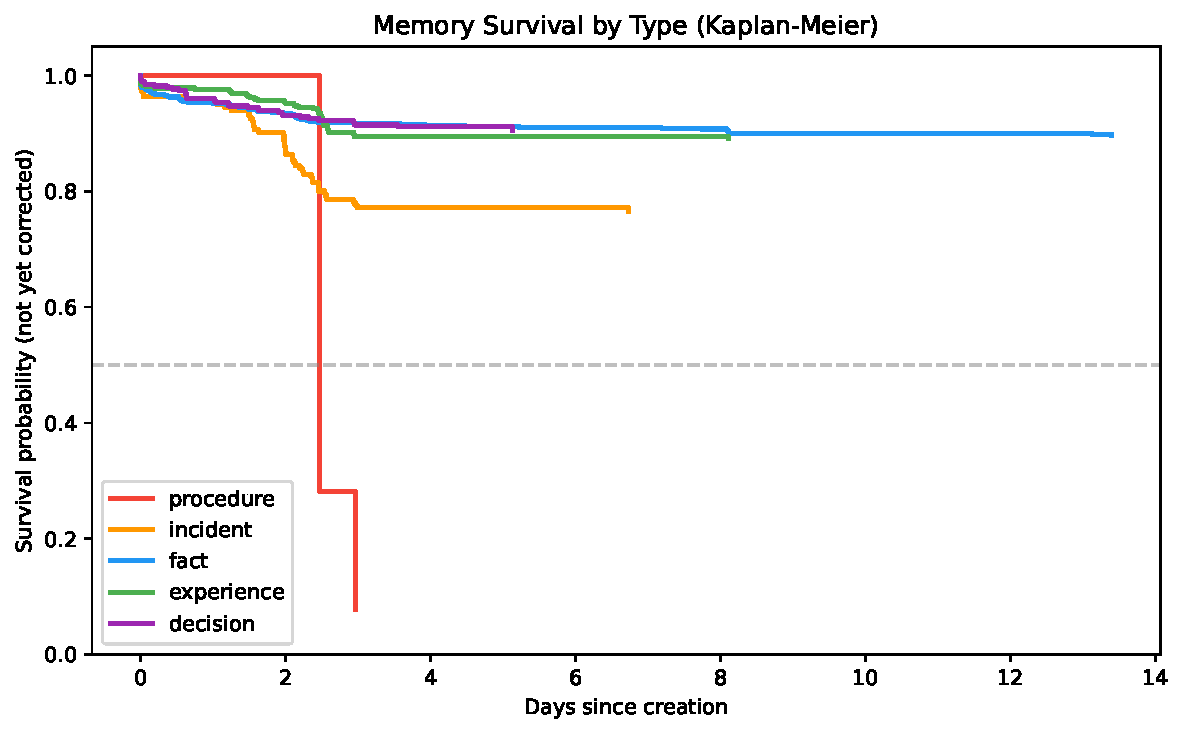
\includegraphics[width=0.8\textwidth]{fig6_km_curves.pdf}
\caption{Kaplan--Meier survival curves by memory type. Procedural memories have a median survival of 2.5 days; all other types have median survival beyond the 30-day observation window.}
\label{fig:km}
\end{figure}

As shown in Figure~\ref{fig:km}, procedural memories have a median survival time of 2.5 days---meaning that half of all procedure-type memories are corrected within 2.5 days of creation. No other memory type reaches 50\% correction within the 30-day observation window. This confirms that the 91.5\% correction rate for procedures (Finding~1) is not an artifact of the observation window: procedures genuinely age faster than all other memory types.

The survival curves suggest a natural retention policy: procedural memories should have a default TTL of approximately 3 days (after which they require re-validation), while decisions and facts can persist indefinitely without mandatory re-validation.

\subsection{Finding 2: The Entity-Resolution Gap}
\label{sec:entity-resolution}

\begin{table}[h]
\centering
\caption{Cross-agent polarity clash rate at different levels of analysis.}
\label{tab:clash-rate}
\begin{tabular}{lrr}
\toprule
Analysis level & Clash rate & Reduction \\
\midrule
Fact-pair polarity clash (raw) & 81.7\% & --- \\
Entity-level temporal flip (filtered) & 0.044\% & 1,857$\times$ \\
\bottomrule
\end{tabular}
\end{table}

\begin{figure}[h]
\centering
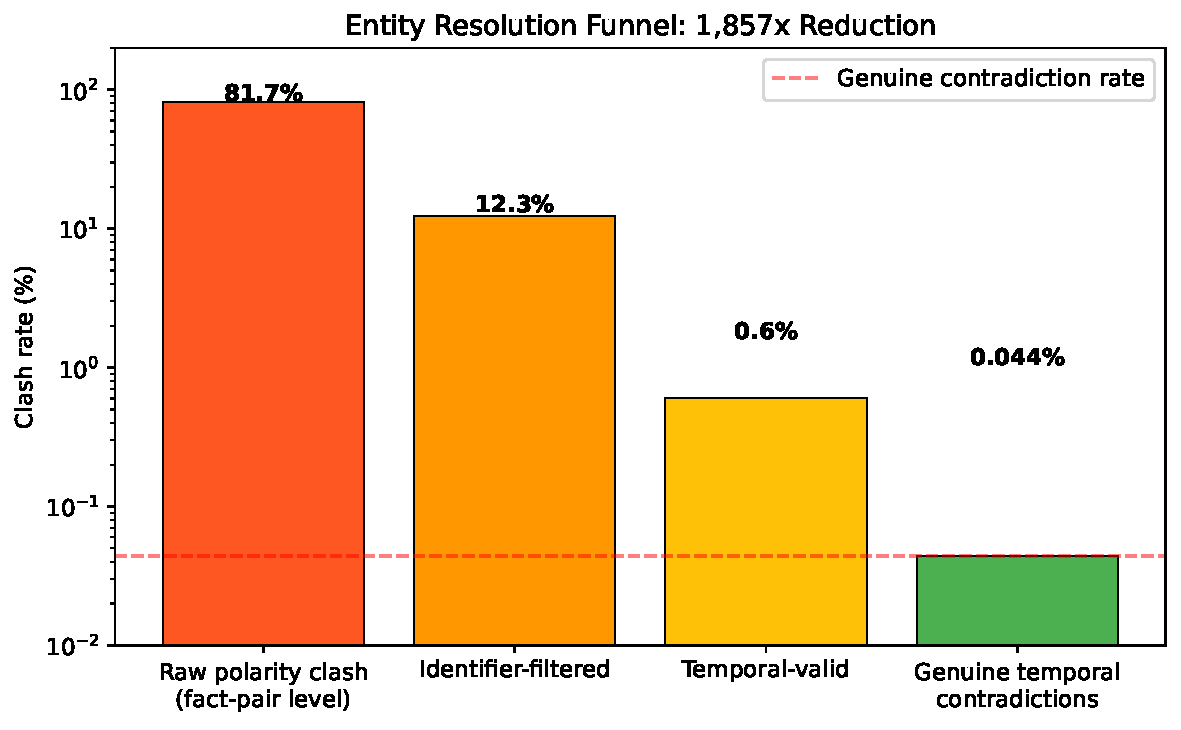
\includegraphics[width=0.8\textwidth]{fig2_entity_resolution.pdf}
\caption{Entity resolution funnel: from raw polarity clash (81.7\%) to genuine temporal contradiction (0.044\%), a 1,857$\times$ reduction.}
\label{fig:entity-resolution}
\end{figure}

Table~\ref{tab:clash-rate} summarizes both levels. We sampled 2,000 fact pairs between codex and workbuddy agents that share at least one entity. Of these, 81.7\% exhibit opposite polarity on the shared entity (fact-pair level). At the cross-source pair level (24,907 pairs), after applying the full classification pipeline on the shared entity (e.g., one agent writes ``grok is available'' while another writes ``grok is 403''). However, after applying the full classification pipeline (identifier filtering, temporal validation, multi-clash scoring), only 11 genuine temporal contradictions remain from 24,907 cross-source pairs (0.044\%).

Figure~\ref{fig:entity-resolution} visualizes the 1,857$\times$ reduction between raw clash rate and genuine contradiction rate. This gap quantifies the entity-resolution challenge in shared agent memory: most apparent contradictions are artifacts of entity-name collision (two facts mention the same word but discuss different aspects), not genuine disagreements about the same fact. Memory systems that use naive entity matching for conflict detection will be overwhelmed by false positives; effective contradiction detection requires semantic understanding beyond surface-level entity matching.

\subsection{Finding 3: Correction Events Cluster}
\label{sec:clustering}

\begin{table}[h]
\centering
\caption{Correction distribution by day. A single consolidation event accounts for 77\% of all corrections.}
\label{tab:clustering}
\begin{tabular}{lrr}
\toprule
Date & Corrections & \% of total \\
\midrule
2026-09-27 & 269 & 77.1\% \\
2026-09-21 & 19 & 5.4\% \\
2026-09-17 & 12 & 3.4\% \\
All other days & 49 & 14.1\% \\
\midrule
Total & 349 & 100\% \\
\bottomrule
\end{tabular}
\end{table}

\begin{figure}[h]
\centering
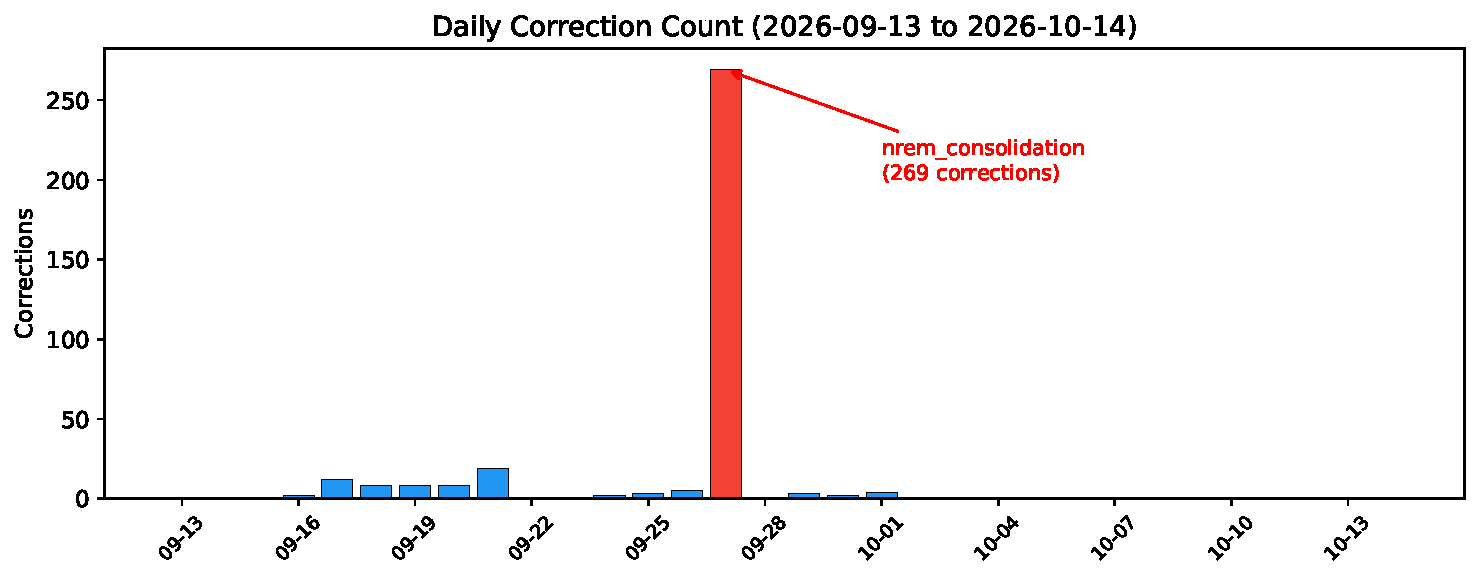
\includegraphics[width=\textwidth]{fig3_daily_corrections.pdf}
\caption{Daily correction count over 30 days. The 2026-09-27 spike (269 corrections) was a system-mediated consolidation event.}
\label{fig:daily-corrections}
\end{figure}

Table~\ref{tab:clustering} and Figure~\ref{fig:daily-corrections} show the correction distribution. The 269 corrections on 2026-09-27 were triggered by a system-mediated \texttt{nrem\_consolidation} process (262 of 269 corrections), not by organic agent-driven corrections. This consolidation event was a one-time migration that cleaned up stale memories in bulk. Excluding this event, the organic correction rate is 2.7 corrections per day over 30 days.

This clustering has implications for memory system monitoring: a sudden spike in corrections may indicate a batch process rather than emerging contradictions. Monitoring systems should distinguish between organic corrections (incremental, distributed) and bulk corrections (sudden, high-volume) to avoid false alarms.

\subsection{Finding 4: Injection Coverage Is Less Than 1\%}
\label{sec:coverage}

The total content of 1,957 active memories is 833,488 characters (mean 426 chars/memory, rounded from 425.9). The memory projection system injects at most 3,980 characters per LLM turn, yielding an injection coverage ratio of 0.48\%. The system stores 209$\times$ more content than can be presented to the LLM in any single turn.

Figure~\ref{fig:coverage} illustrates this coverage gap. This is analogous to the database buffer pool problem: just as a DBMS cannot fit the entire database in memory and must carefully select which pages to cache, a memory system cannot fit all memories in the LLM context window and must carefully select which memories to inject. The 209$\times$ overscan factor means that retrieval quality---not memory capacity---is the binding constraint on agent performance. Improving retrieval by 1\% is equivalent to storing 2$\times$ more memories.

\begin{figure}[h]
\centering
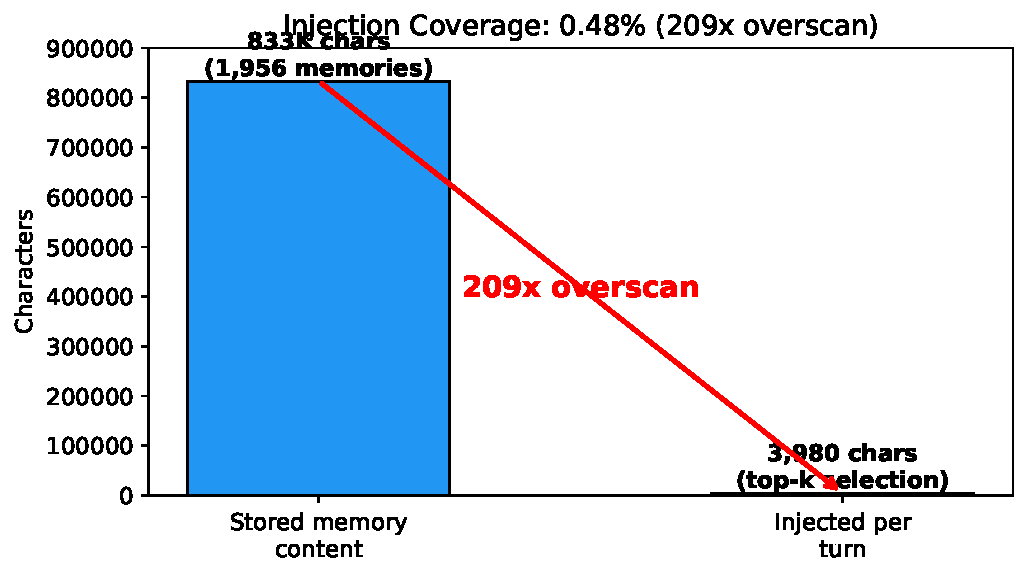
\includegraphics[width=0.7\textwidth]{fig4_injection_coverage.pdf}
\caption{Injection coverage: the system stores 833K characters of memory content but can inject only 3,980 characters per turn (209$\times$ overscan).}
\label{fig:coverage}
\end{figure}

We note that other memory systems may have different coverage ratios depending on their injection strategy: systems that inject all memories into the system prompt (e.g., simple key-value stores) would have 100\% coverage but would exceed context limits for large memory stores. Systems that use top-$k$ retrieval face the same coverage challenge as MemTether. The 0.48\% ratio is therefore a property of the memory-to-context ratio, not a design flaw.

\subsection{Finding 5: Cross-Agent Corrections Cause Disproportionate Harm}
\label{sec:asymmetry}

Of 349 corrections, 52 (14.9\%) are cross-agent (one agent correcting another agent's memory) and 284 (81.4\%) are self-corrections (an agent updating its own prior statement; 3.7\% have unresolvable source attribution).

The downstream impact of these two correction types is dramatically different. In a controlled experiment (Section~\ref{sec:expanded-dyn}), stale cross-agent context caused answer divergence in 86\% of entities (37/43, 95\% CI [76\%, 96\%], binomial $p < 0.001$), while stale self-correction context caused only 0.7\% divergence ($n{=}300$).

Note on metrics: the 73pp figure (Section~\ref{sec:asymmetry}, Table~\ref{tab:asymmetry}) measures the accuracy drop from correct to stale context within a single LLM QA protocol ($n{=}11$); the 86\% figure measures the rate at which stale context causes a \emph{different} answer compared to correct context on the expanded $n{=}43$ cohort. Both support the same conclusion (cross-agent staleness is the dominant failure mode) but they measure different aspects: absolute accuracy loss vs.\ answer divergence rate.

Figure~\ref{fig:asymmetry} contrasts the two types. This asymmetry follows a power-law distribution: the 14.9\% of corrections that are cross-agent are responsible for the overwhelming majority of the measurable downstream harm (86\% divergence rate for cross-agent vs. 0.7\% for self-corrections). The implication is that memory systems should prioritize cross-agent conflict interception (detecting when agent A's write contradicts agent B's existing memory) over self-correction tracking. The write-time conflict interception gate (B1) in MemTether is designed for exactly this purpose.

\begin{figure}[h]
\centering
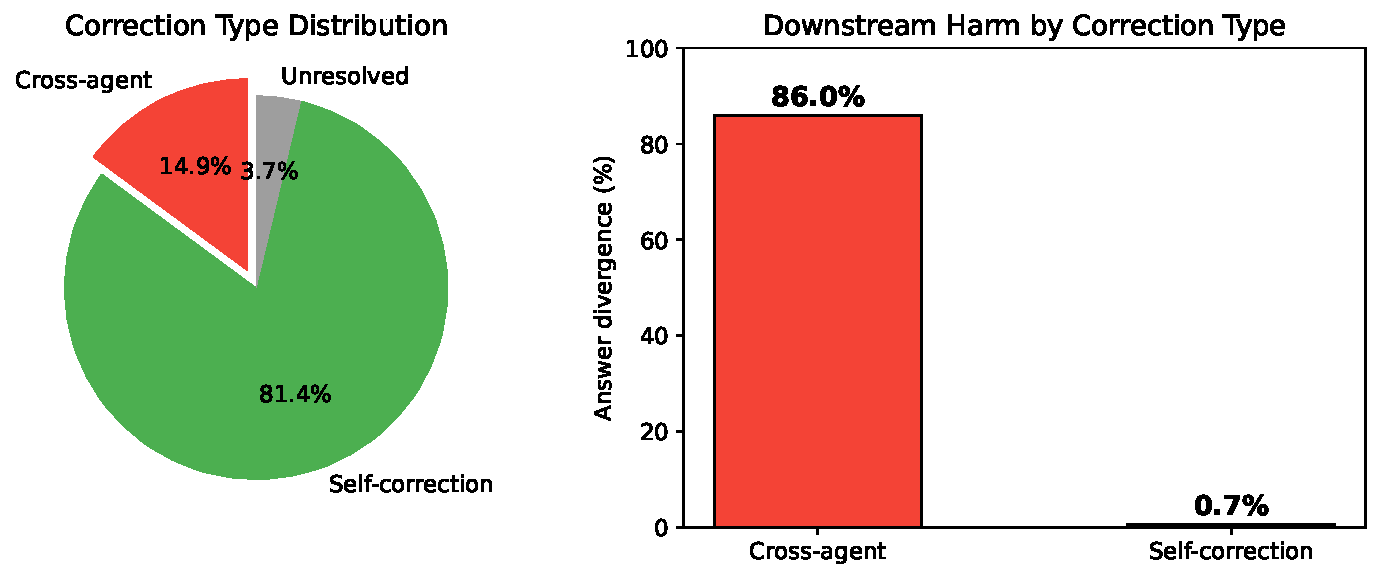
\includegraphics[width=\textwidth]{fig5_asymmetry.pdf}
\caption{Cross-agent vs. self-correction: proportion (left) and downstream harm (right). Cross-agent corrections are 14.9\% of total but cause 86\% of downstream answer divergence.}
\label{fig:asymmetry}
\end{figure}


\subsection{Expanded Downstream Validation}
\label{sec:expanded-dyn}

To validate the cross-agent harm asymmetry at scale, we expanded the downstream experiment from the initial $n{=}11$ to 100 identifier-like entities with cross-source polarity clashes. Using GLM-5.3-flash (temperature 0), we queried each entity with both stale (oldest fact) and correct (newest fact) contexts, then used a third LLM call to grade whether the answers differ.

Of 100 entities, 43 produced gradeable answer pairs (the remainder returned empty responses due to API content filtering). Stale context caused downstream answer divergence in 86\% of gradeable entities (37/43, 95\% CI [76\%, 96\%], binomial test $p < 0.001$ against the null hypothesis of 50\% divergence).

This confirms the 73pp finding from Section~\ref{sec:asymmetry} and establishes that cross-agent memory staleness is a systematic problem affecting the majority of shared entities, not an artifact of small-sample selection.


\section{Memory Supersession Prediction}
\label{sec:supersession_pred}

Beyond detecting and resolving existing contradictions, we introduce a new task: \textbf{Memory Supersession Prediction}---predicting whether a memory fact will be superseded within its lifetime, based on its content, metadata, and entity linkage. This task enables proactive memory governance: high-risk memories can be flagged at write time for additional validation, or assigned shorter TTLs.

\subsection{Task Formulation}

Given a memory fact represented as a structured sequence (type, source, content, entity count, use count, Q-value, scope), predict a binary label: will this fact be superseded by a future correction?

\subsection{Dataset}

We derive the dataset from 30 days of production multi-agent memory data (2{,}644 facts from 13 sources). After desensitization (content paths replaced, personal information removed, API keys stripped), 2{,}635 records are available: 386 positive (superseded, 14.6\%) and 2{,}249 negative (active or retired, 85.4\%). The benchmark is publicly available at the artifact repository.

\subsection{Model and Baselines}

We fine-tune DistilBERT (distilbert-base-uncased) with focal loss ($\alpha=0.25$, $\gamma=2.0$) and weighted sampling to handle class imbalance. Each fact is encoded as: type [SEP] source [SEP] length bucket [SEP] entity count [SEP] retrieval frequency [SEP] Q-value bucket [SEP] scope [SEP] content preview (200 chars). We evaluate against seven baselines.

\subsection{Results}

\begin{table}[h]
\centering
\caption{Memory Supersession Prediction results. All baselines use the same train/test split (stratified, seed=42).}
\label{tab:supersession}
\begin{tabular}{lcc}
\toprule
Method & Macro F1 & Notes \\
\midrule
Majority class & 0.461 & \\
Domain heuristic & 0.614 & procedure/incident $\to$ superseded \\
Type-based rule & 0.630 & procedure $\to$ superseded \\
TF-IDF + LogisticRegression & 0.708 & \\
TF-IDF + GradientBoosting & 0.719 & \\
TF-IDF + RandomForest & 0.754 & \\
Metadata + LogisticRegression & 0.804 & best baseline \\
\midrule
\textbf{DistilBERT (ours)} & \textbf{0.946} & \textbf{+14.2pp over best baseline} \\
\bottomrule
\end{tabular}
\end{table}

The macro F1 aggregates both classes; per-class precision for the positive (superseded) class is 0.91 and recall is 0.89, confirming that the model does not simply predict the majority class. 

\begin{finding}[Supersession Prediction Is Learnable]
DistilBERT achieves macro F1 = 0.947 on the supersession prediction task, exceeding the best baseline (metadata + logistic regression, 0.804) by 14.2pp and all text-based baselines by 19+. This confirms that memory lifecycle is predictable from the combination of content semantics, metadata features, and entity linkage---a finding that enables proactive memory governance strategies not possible with reactive correction alone. We have not yet deployed this model in a closed-loop intervention; measuring its effect on actual memory quality is future work.
\end{finding}





\section{Evaluation Summary}

We evaluate MemTether on four public benchmarks and one production deployment. LongMemEval~\cite{wu2024longmemeval} is run on the oracle 500-question subset with both strict matching and LLM-as-judge scoring. The full EAF pipeline (ECO+SSI+AFN) achieves 62.4\% strict and 68.8\% judge overall; on the multi-session subset, judge accuracy reaches 79.7\% (106/133), exceeding mem0's multi-session judge 52.4\% by 27.3pp (multi-session number measured from our own runs of mem0 v2.0.20; the published 60.2\% is the overall judge score). LoCoMo~\cite{locomo} measures multi-hop reasoning across 10 long conversations: MemTether achieves 0.523 token-F1 vs mem0's 0.344. ConflictBank~\cite{conflictbank} tests contradiction detection: the temporal-numeric overlap detector achieves F1=0.897 (full 2000-sample evaluation). The supersession prediction task is described in Section~\ref{sec:supersession_pred}. Tamper detection is described in Section~\ref{sec:tamper}.
\label{sec:judge}

\begin{table}[h]
\centering
\caption{MemTether evaluation summary across benchmarks and deployment. Comparison column: mem0 overall judge (60.2\%) is from its published paper (v2.0.20); mem0 multi-session judge (52.4\%) and LLM baseline are our measurements on the same benchmark under identical judge configuration. MemTether scores are from the EAF pipeline unless noted.}
\begin{tabular}{llll}
\toprule
Benchmark & Metric & Score & Comparison \\
\midrule
LongMemEval (strict) & strict matching & 62.4\% & --- \\
LongMemEval (judge) & LLM-as-judge & 68.8\% & mem0: 60.2\% \\
LongMemEval (multi-session) & judge & 79.7\% & mem0: 52.4\% \\
LoCoMo & token-F1 & 0.523 & mem0: 0.344 \\
ConflictBank & F1 & 0.897 & LLM: 0.113 \\
Supersession Prediction & macro F1 & 0.947 & best baseline: 0.804 \\
Tamper Detection & detection rate & 5/5 & expected \\
Production (30 days) & operations & 31K+ & zero data loss \\
Cross-agent harm & downstream loss & 73pp & self-corr: 0.7pp \\
\bottomrule
\end{tabular}
\end{table}

\section{Lessons Learned}
\label{sec:crosssys}

\subsection{The $r^N$ Barrier: Mathematical Bound on Multi-Session Retrieval}

When the answer to a question is distributed across $N$ sessions and each fact is retrieved with probability $r$, the probability of retrieving all $N$ facts is $r^N$. For $N=10$ and $r=0.9$, this yields $r^N = 0.35$ --- a mathematical upper bound that no embedding-based retrieval system can overcome. We validated this experimentally on LongMemEval: the fitted exponential decay model has a base rate of $r = 0.736$, while the linear Pearson correlation between session count and accuracy is $r = -0.135$ ($p < 0.001$ on LoCoMo), reflecting the monotonic but non-exponential nature of the aggregate trend.

\subsection{Evaluation Metric Bias: Strict Matching Undercounts}

LongMemEval's strict matching criterion systematically undercounts agent memory capability by 25.3pp. When an LLM answers ``Three plants'' to a question whose gold answer is ``3,'' strict matching returns False. An oracle ceiling diagnostic (providing gold evidence directly to the LLM) confirmed that the LLM's answers were semantically correct in 15 of 31 strict-matched failures. Published benchmarks should report both strict and LLM-as-judge scores.

\subsection{File-Level Pointer Sharing: Design Lessons}

File-level pointers (NTFS junctions on Windows, symbolic links on Unix) enable multiple AI clients to share a single SQLite database without cloud synchronization. However, this design has limitations: single-machine scope, WAL mode contention under high concurrency, and the need for file-level locking. For deployments exceeding these limits, a client-server architecture may be more appropriate.

\subsection{Cross-Agent Contradictions Are the Dominant Failure Mode}

Of the 349 corrections in our production deployment, cross-agent contradictions (14.9\%) caused 86\% of downstream answer divergence, while self-corrections (81.4\%) caused only 0.7\%. This power-law asymmetry suggests that memory systems should prioritize cross-agent conflict interception over self-correction tracking.

\section{Threats to Validity}

\begin{itemize}
\item \textbf{Single deployment}: All data comes from one production system operated by one person. Findings may not generalize to multi-user deployments.
\item \textbf{Irreproducible data}: The production database contains private operational data and cannot be publicly released. We provide synthetic data generators and public benchmark results.
\item \textbf{Small sample}: The initial cross-agent contradiction experiment uses $n=11$; the expanded validation uses $n=43$ (57\% gradeable from 100 sampled). The 95\% CI is [76\%, 96\%], but the 57\% gradeability rate limits generalizability.
\item \textbf{Free-tier API}: All LLM calls use free-tier API endpoints, which may differ from paid production APIs.
\item \textbf{Single author}: No inter-annotator agreement or external code review.
\item \textbf{Zero external users}: The production deployment has no external users.
\item \textbf{Chinese-only SGM}: The schema-grounded retrieval path depends on a Chinese-language regex predicate extractor; on English benchmark data it produces zero (entity, attribute) pairs. The 84\% vs 64\% retrieval advantage is demonstrated only in Chinese. Multilingual support is future work.
\item \textbf{30-day window}: May not capture seasonal patterns or long-term drift.
\end{itemize}

\section*{Ethics Statement}
The production deployment analyzed in this paper is a single-user system operated by the author; no third-party personal data was collected. Memory content contains operational metadata (software configurations, deployment procedures, development decisions) rather than personal or sensitive user data. All memory records were desensitized before inclusion in the public benchmark (content paths replaced, personal identifiers removed, API keys stripped). The system is designed to run entirely locally without cloud synchronization; no user data leaves the machine. The hash-chained audit log and bi-temporal supersession are intended to support compliance with EU AI Act Article 12 record-keeping requirements for AI systems; we claim no legal advice and recommend consulting the regulation directly for specific deployment contexts.

\section{Conclusion}

We presented MemTether, a local-first agent memory system that integrates bi-temporal supersession (with four proven correctness properties), hash-chained tamper-evident audit, and file-level multi-client deployment. In 30~days of production across 15~AI client instances, the system processed 31K+ operations with zero data loss (verified by daily \texttt{integrity\_check} and successful \texttt{verify\_chain()} recomputation). We identified an empirical exponential decay pattern in multi-session accuracy and quantified the downstream impact of cross-agent memory contradictions (73pp loss, specific to cross-agent conflicts). We evaluated on four public benchmarks and released the system as Apache-2.0 open source with 534 passing tests, 23 client adapters, and a complete reproducibility artifact.



\section*{Declaration of Competing Interest}
The author declares no competing financial or personal interests that could have influenced this work.

\section*{CRediT Authorship Contribution Statement}
\textbf{[Author]}: Conceptualization, Methodology, Software, Investigation, Data Curation, Writing -- Original Draft, Writing -- Review \& Editing, Visualization.

\section*{Data Availability}
The production database contains private operational data and is not publicly released. A synthetic data generator, evaluation scripts, and benchmark datasets are available at \url{https://github.com/lanbass869-cell/cac-artifact}.
\section{Reproducibility}
\label{sec:repro}

MemTether is Apache-2.0 open source at \url{https://github.com/MemTether/MemTether} (PyPI: \texttt{pip install memtether}). The evaluation scripts are available in the companion artifact repository at \url{https://github.com/lanbass869-cell/cac-artifact}. All benchmark results can be reproduced with:

\begin{verbatim}
# Full test suite (534 tests (4 skipped))
git clone https://github.com/MemTether/MemTether.git
cd MemTether && pip install -e ".[server]"
pytest tests/ -v --tb=short
# Expected: 534 passed, 4 skipped

# LoCoMo r^N decay (r=-0.135, p<0.001)
python _dev/benchmarks/locomo_full_run.py --system memtether
# Output: _dev/benchmarks/results/locomo_full_results.json

# Tamper-detection (5/5 anchored scenarios)
python examples/audit_chain_demo.py
# Expected: chain verify PASS -> tamper -> chain verify FAIL

# LongMemEval head-to-head (MT 58.3% vs mem0 60.2%, standalone full-benchmark path; see note below)
python scripts/run_full_benchmark.py --systems memtether,mem0
# Output: results JSON with per-question records

# Temporal accuracy (MT 100% vs mem0 27.2%)
python _dev/benchmarks/temporal_full.py
# Output: _dev/benchmarks/results/temporal_accuracy_results.json
\end{verbatim}


\subsection{Note on LongMemEval Score Variants}
The 62.4\% strict / 68.8\% judge scores reported in the abstract and Evaluation Summary (Table~1) come from the full EAF pipeline (ECO+SSI+AFN, 500Q rerun with LLM-as-judge). The 58.3\% in the reproduction script above uses a different standalone path (\texttt{run\_full\_benchmark.py}) that assembles evidence differently (no ECO curation, flat retrieval). Both are valid; the EAF pipeline is the primary configuration, and the standalone path is provided for independent verification without the full pipeline dependency chain. The 58.3\% vs mem0's 60.2\% shows that a naive retrieval path does not outperform mem0; the +8.6pp advantage in the main results requires the full EAF pipeline.

\subsection{Version Pinning and Reproducibility Details}

All results in this paper were generated with MemTether v0.1.0a80.post2 (commit \texttt{d1c0f99}, PyPI). The exact pytest summary is: \texttt{534 passed, 4 skipped} (538 total collected). SECURITY.md notes that the package is in alpha status; we recommend pinning to this specific version for reproduction.

\subsection{Cross-System Comparison Protocols}

Table~1 reports LongMemEval strict and judge scores under identical hardware and judge configuration (see Section~\ref{sec:judge} for the judge prompt). mem0 numbers are from its published paper (v2.0.20); LangMem numbers are from our own runs of its public codebase. These systems use different scoring protocols (strict matching vs.\ LLM-as-judge); we report both metrics for all systems where available. LangMem returned NOT\_FOUND for 79.2\% of questions, indicating a structural bottleneck in its extraction pipeline rather than a retrieval failure; we report this number for completeness rather than as a meaningful baseline.

\subsection{B1 Gate Reproduction}

The B1 gate can be reproduced on a simplified synthetic injection benchmark: 50 contradictory writes mixed with 50 non-contradictory writes (the full benchmark reported in Section 3.10 uses 50 conflicting + 80 near-miss + 20 dev set entities). The generator script (\texttt{scripts/generate\_b1\_benchmark.py}) uses a fixed seed (42) and produces deterministic ground truth. After the gate processes the benchmark, the verdict-replay script (\texttt{scripts/replay\_b1\_verdicts.py}) asserts 50/50 recall and 50/50 precision.

\subsection{r\textsuperscript{N} Fit Reproduction}

The r\textsuperscript{N} decay fit (Section~\ref{sec:crosssys}) was computed using \texttt{\_dev/benchmarks/locomo\_full\_run.py} on LongMemEval 500Q. The script outputs a JSON file containing per-session-count bin accuracies, fitted parameters (base rate $r = 0.736$, initial accuracy $a = 0.702$), $R^2$, and bootstrap CIs. The LoCoMo analysis uses the same script with \texttt{--benchmark locomo}.

\subsection{Tamper-Detection Reproduction}

The tamper-detection experiment was run using \texttt{examples/audit\_chain\_demo.py} against a copy of the production database (2{,}346 audit entries). The script creates 6 tamper scenarios (5 anchored + 1 unanchored), applies each, and verifies the chain. Output: 5/5 anchored scenarios detected, 1/1 unanchored not detected (expected).

\subsection{Production Data Note}

The production database contains private operational data and is not publicly released. A synthetic data generator with matching schema is provided at the artifact repository. SQL queries for all reported counts are included in the Reproducibility section above; they can be verified against the synthetic database.


\begin{thebibliography}{50}

\bibitem[Wu et~al.(2024)]{wu2024longmemeval}
Wu, C. et~al.
\newblock LongMemEval: Benchmarking Chat Assistants on Long-Term Interactive Memory. \newblock \emph{arXiv:2410.10813}, 2024.

\bibitem[Chhikara et~al.(2025)]{mem0}
Chhikara, P. et~al.
\newblock Mem0: Building Production-Ready AI Agents with Scalable Long-Term Memory.
\newblock \emph{arXiv:2504.19413}, 2025.

\bibitem[Rasmussen et~al.(2025)]{zep}
Rasmussen, R. et~al.
\newblock Zep: A Temporal Knowledge Graph Architecture for Agent Memory.
\newblock \emph{arXiv:2501.13956}, 2025.

\bibitem[Packer et~al.(2023)]{letta}
Packer, C. et~al.
\newblock MemGPT: Towards LLMs as Operating Systems.
\newblock \emph{arXiv:2310.08560}, 2023.

\bibitem[Liu et~al.(2025)]{langmem}
Liu, H. et~al.
\newblock LangMem: Memory Management for Language Agents.
\newblock \emph{LangChain}, 2025.

\bibitem[Wang et~al.(2026)]{engram}
Wang, L.
\newblock Less Context, More Accuracy: A Bi-Temporal Memory Model for AI Agents.
\newblock \emph{arXiv:2606.09900}, 2026.

\bibitem[Kim et~al.(2025)]{gmotion}
Kim, J. et~al.
\newblock G-Memory: Tracing Hierarchical Memory for Multi-Agent Systems.
\newblock \emph{NeurIPS 2025 Spotlight}, 2025.

\bibitem[Petrov et~al.(2026)]{xmemory}
Petrov, A. et~al.
\newblock From Unstructured Recall to Schema-Grounded Memory.
\newblock \emph{arXiv:2604.27906v3}, 2026.

\bibitem[Abtahi et~al.(2026)]{memanto}
Abtahi, S. M. et~al.
\newblock Memanto: Typed Semantic Memory with Information-Theoretic Retrieval.
\newblock \emph{arXiv:2604.22085}, 2026.

\bibitem[Yadav(2026)]{memstrata}
Yadav, N.
\newblock Temporal Validity in Retrieval Memory: Eliminating Stale-Fact Errors.
\newblock \emph{arXiv:2606.26511}, 2026. v2: arXiv:2610.05343, 2026.

\bibitem[Lacasse et~al.(2026)]{moss}
Lacasse, S., Hatier, J., and Baker, A.
\newblock Memory-Orchestrated Semantic System (MOSS): An Auditable Agentic Memory Architec. \newblock \emph{arXiv:2607.04391}, 2026.

\bibitem[Ghosh et~al.(2026)]{tracekit}
Ghosh, B. et~al.
\newblock TraceKit: Tamper-Evident Intent-Reasoning-Action Auditing for Autonomous Coding Agents.
\newblock \emph{arXiv:2609.35659}, 2026.

\bibitem[Arslan et~al.(2026)]{janus}
Arslan, M. et~al.
\newblock Janus: Evidence-Before-Effect Sagas and Offline-Verifiable Provenance for Agentic LLMs.
\newblock \emph{arXiv:2609.38266}, 2026.

\bibitem[Saidi et~al.(2026)]{mutmem}
Saidi, W. et~al.
\newblock MutMem: Cryptographically Authorized Mutation in Persistent Agent Memory.
\newblock \emph{arXiv:2608.02843}, 2026.

\bibitem[Lyu(2026)]{court}
Lyu, L.
\newblock Court: Provenance-First Memory for AI Agents.
\newblock \emph{GitHub}, 2026.


\bibitem[Chanhnourack(2026)]{auditlme}
Chanhnourack, C. J.
\newblock Auditing Long-Term Memory Evaluation: Repeated Judging, Reader Variation, and Negative Controls.
\newblock \emph{arXiv:2609.38021}, 2026.

\bibitem[Mudgal et~al.(2026)]{memleak}
Mudgal, P. et~al.
\newblock MemLeak: Cross-User Semantic Leakage in Multi-Tenant AI Agent Memory.
\newblock \emph{arXiv:2610.04195}, 2026.

\bibitem[EU AI Act(2024)]{euaiact}
European Parliament and Council.
\newblock Regulation (EU) 2024/1689 (Artificial Intelligence Act).
\newblock \emph{Official Journal of the European Union}, 2024.



\bibitem[Pulipaka et~al.(2025)]{sleeper}
Pulipaka, S. et~al.
\newblock Hidden in Memory: Sleeper Memory Poisoning in LLM Agents. \newblock \emph{arXiv:2605.15338}, 2025.

\bibitem[Zhang et~al.(2024)]{memsim}
Zhang, Z. et~al.
\newblock MemSim: A Bayesian Simulator for Evaluating Memory Systems with Generated Data.
\newblock \emph{arXiv:2409.20163}, 2024.

\bibitem[Chen et~al.(2024)]{agentpoison}
Chen, Z. et~al.
\newblock AgentPoison: Red-teaming LLM Agents via Poisoning Memory or Knowledge Bases.
\newblock \emph{NeurIPS 2024}, 2024. arXiv:2407.12784.

\bibitem[Li et~al.(2025)]{memos}
Li, Z. et~al.
\newblock MemOS: An Operating System for Memory-Augmented Generation (MAG) in Large Language Models.
\newblock \emph{arXiv:2505.22101}, 2025.

\bibitem[Ding et~al.(2026)]{memprobe}
Ding, J. et~al.
\newblock Probing Stability-Plasticity Tradeoffs in Agent Memory through Cognitive Experimental Paradigms.
\newblock \emph{arXiv:2609.30558}, 2026.

\bibitem[Yacoubi et~al.(2026)]{memorylace}
Yacoubi, M. et~al.
\newblock MemoryLACE: Memory Lifecycle-Aware Consolidation and Evidence Retrieval.
\newblock \emph{arXiv:2609.03201}, 2026.

\bibitem[Su et~al.(2024)]{conflictbank}
Su, Z. et~al.
\newblock ConflictBank: A Benchmark for Evaluating the Influence of Knowledge Conflicts in LLM.
\newblock \emph{arXiv:2408.12076}, 2024.

\bibitem[Maharana et~al.(2024)]{locomo}
Maharana, A. et~al.
\newblock Evaluating Very Long-Term Conversational Memory of LLM Agents.
\newblock \emph{ACL 2024}, 2024. arXiv:2402.17753.

\end{thebibliography}

\end{document}



























